\documentclass[review]{elsarticle}

\usepackage{lineno,hyperref}
\usepackage{multirow}
\usepackage{multicol}
\usepackage{amsmath}
\usepackage[ruled]{algorithm2e}
\usepackage{subfigure}
\usepackage{xcolor}
\usepackage{amssymb}

\modulolinenumbers[5]
 
\journal{Journal of \LaTeX\ Templates}

%%%%%%%%%%%%%%%%%%%%%%%
%% Elsevier bibliography styles
%%%%%%%%%%%%%%%%%%%%%%%
%% To change the style, put a % in front of the second line of the current style and
%% remove the % from the second line of the style you would like to use.
%%%%%%%%%%%%%%%%%%%%%%%

%% Numbered
%\bibliographystyle{model1-num-names}

%% Numbered without titles
%\bibliographystyle{model1a-num-names}

%% Harvard
%\bibliographystyle{model2-names.bst}\biboptions{authoryear}

%% Vancouver numbered
%\usepackage{numcompress}\bibliographystyle{model3-num-names}

%% Vancouver name/year
%\usepackage{numcompress}\bibliographystyle{model4-names}\biboptions{authoryear}

%% APA style
%\bibliographystyle{model5-names}\biboptions{authoryear}

%% AMA style
%\usepackage{numcompress}\bibliographystyle{model6-num-names}

%% `Elsevier LaTeX' style
\bibliographystyle{elsarticle-num}
%%%%%%%%%%%%%%%%%%%%%%%

\begin{document}

\begin{frontmatter}

\title{Deep Reinforcement Learning based Bagging Model for Rumor Tracking}

%% Group authors per affiliation:
\author{Ming Dong$^1$, Guohui Li$^1$, Lingfeng Ming$^1$, Changyin Luo$^2$,\\Han Yu$^3$, Xiaofei Hu$^3$, Bolong Zheng$^1$\corref{mycorrespondingauthor}}
\address{$^1$Huazhong University of Science and Technology, Wuhan, China}
\address{$^2$Central China Normal University, Wuhan, China}
\address{$^3$Wuhan Fiberhome Technical Services Co.,Ltd, Wuhan, China}

\cortext[mycorrespondingauthor]{Corresponding author: Bolong Zheng}

\begin{abstract} 
Rumor defeating in a fully automated way is a meaningful task for reducing the hazards of rumors in social networks. Usually, content-based rumor defeating is a pipeline task that could be divided into four sub-tasks: detection, tracking, stance classification, and veracity. Compared to the other three sub-tasks, rare studies are dedicated to rumor tracking.  Rumor tracking in social networks is an important sub-task in rumor defeating, which gathers the relevant posts and filters the irrelevant posts for a given rumor news. SOTA work treats rumor tracking as an auxiliary task in multi-task learning and lacks special optimization for it, which limits the accuracy of tracking performance. Consequently, we propose an aggregated model for rumor tracking specifically named ART. By adopting multiple components for different tweets features, we improve the tracking accuracy. Finally, we conduct experiments on public datasets and the experimental results shows the superior of ART on efficiency and effectiveness.
\end{abstract}

\begin{keyword}
rumor tracking\sep natural language processing \sep deep learning \sep multi-task learning
\end{keyword}

\end{frontmatter}

\linenumbers

\section{Introduction}
\label{sec:introduction}
The high-speed development of social networks brings explosive scale of information. The convenience of the social networks accelerates the diffusion of information. People create and publish messages without any limitations, which leads to the widespread dissemination of rumors in social networks \cite{DBLP:journals/corr/KurkaGZ15, DBLP:journals/csur/ZubiagaABLP18, DBLP:conf/sirocco/KostkaOW08, vosoughi2018spread}. Rumors usually appear with unjudged veracity and contain substantive misinformation, which may cause huge damage to the society. For instance, a large number of rumors arise during the COVID-19 epidemic, such as ``More than ten thousand people die in Wuhan." and ``Liquor kills the virus.", causing great public panic. Therefore, it is an urgent task to defeat rumors in social networks.

Social media generates huge amounts of data all the time. It is impracticable to manually defeat rumors on such data scalability. Therefore, many studies have been proposed and can be divided into two categories: diffusion-based rumor source identification and content-based rumor detection. Diffusion-based rumor source identification aims to locate the sources of the rumor at the early stage of rumor diffusion \cite{DBLP:conf/sigmetrics/ShahZ10, DBLP:journals/tit/ShahZ11, DBLP:conf/kdd/LappasTGM10}. Content-based rumor detection aims to judge the veracity of tweet sequences. As shown in Fig.\ref{fig:pipeline}, this task is a pipeline that consists of four sub-tasks \cite{DBLP:journals/csur/ZubiagaABLP18, DBLP:conf/coling/KochkinaLZ18}: rumor detection, rumor tracking, sentence classification, and veracity classification. Rumor detection is to determine whether a tweet sequence is a rumor  \cite{DBLP:conf/socinfo/ZubiagaLP17, DBLP:conf/www/Ma0W19,DBLP:conf/naacl/NguyenDCD19, DBLP:journals/corr/abs-1906-05659}. Sentence classification is to judge the emotion of a tweet sentence \cite{DBLP:conf/semeval/EnayetE17, DBLP:conf/semeval/X17a, DBLP:conf/coling/ZubiagaKLPL16}. Rumor veracity is to determine if a tweet tells the truth \cite{DBLP:conf/coling/KochkinaLZ18, DBLP:conf/acl/LiZS19, DBLP:conf/acl/KumarC19}. These three sub-tasks have attracted extensive attention in recent years. However, only a few studies have been proposed for the rumor tracking task.

Rumor tracking is to collect relevant tweets of a given rumor event. It can be considered to a binary classification problem that classifies the posts to be related or unrelated. However, the existing proposals \cite{DBLP:conf/emnlp/QazvinianRRM11, DBLP:conf/www/ChengNB20}  only consider rumor tracking as an auxiliary task in multi-task learning without special optimization, hence restraining the accuracy of tracking performance.
Therefore, we propose a model that improves the weakness of the existing work for rumor tracking.

The main contributions of this work are summarized as follows:
\begin{itemize}
	\item By exploring plenty of basic models, we proposed an aggregated model named RL-BRT to solve the rumor tracking task. 
	\item We analyze the rumor tracking task and find suitable features and embedding methods. Also, we propose a reinforcement learning based bagging algorithm to aggregate basic models into a macrocosm.
	\item We conduct experiments on public benchmark datasets, and the experimental results show the rationality and superiority of RL-BRT.
\end{itemize}

The rest of this article is structured as follows. In Section \ref{sec:related}, we introduce important works related to RL-BRT. In Section \ref{sec:perliminary}, we introduce some notations and background knowledge of this work. Our proposed model RL-BRT is introduced in Section \ref{sec:model}. Then, Section \ref{sec:experiment} shows the experimental settings and results. Finally, we give the conclusion and future work in Section \ref{sec:conclusion}.

\begin{figure}[tbp]
	\hspace{0ex}
	\vspace{0ex}
	\centering
	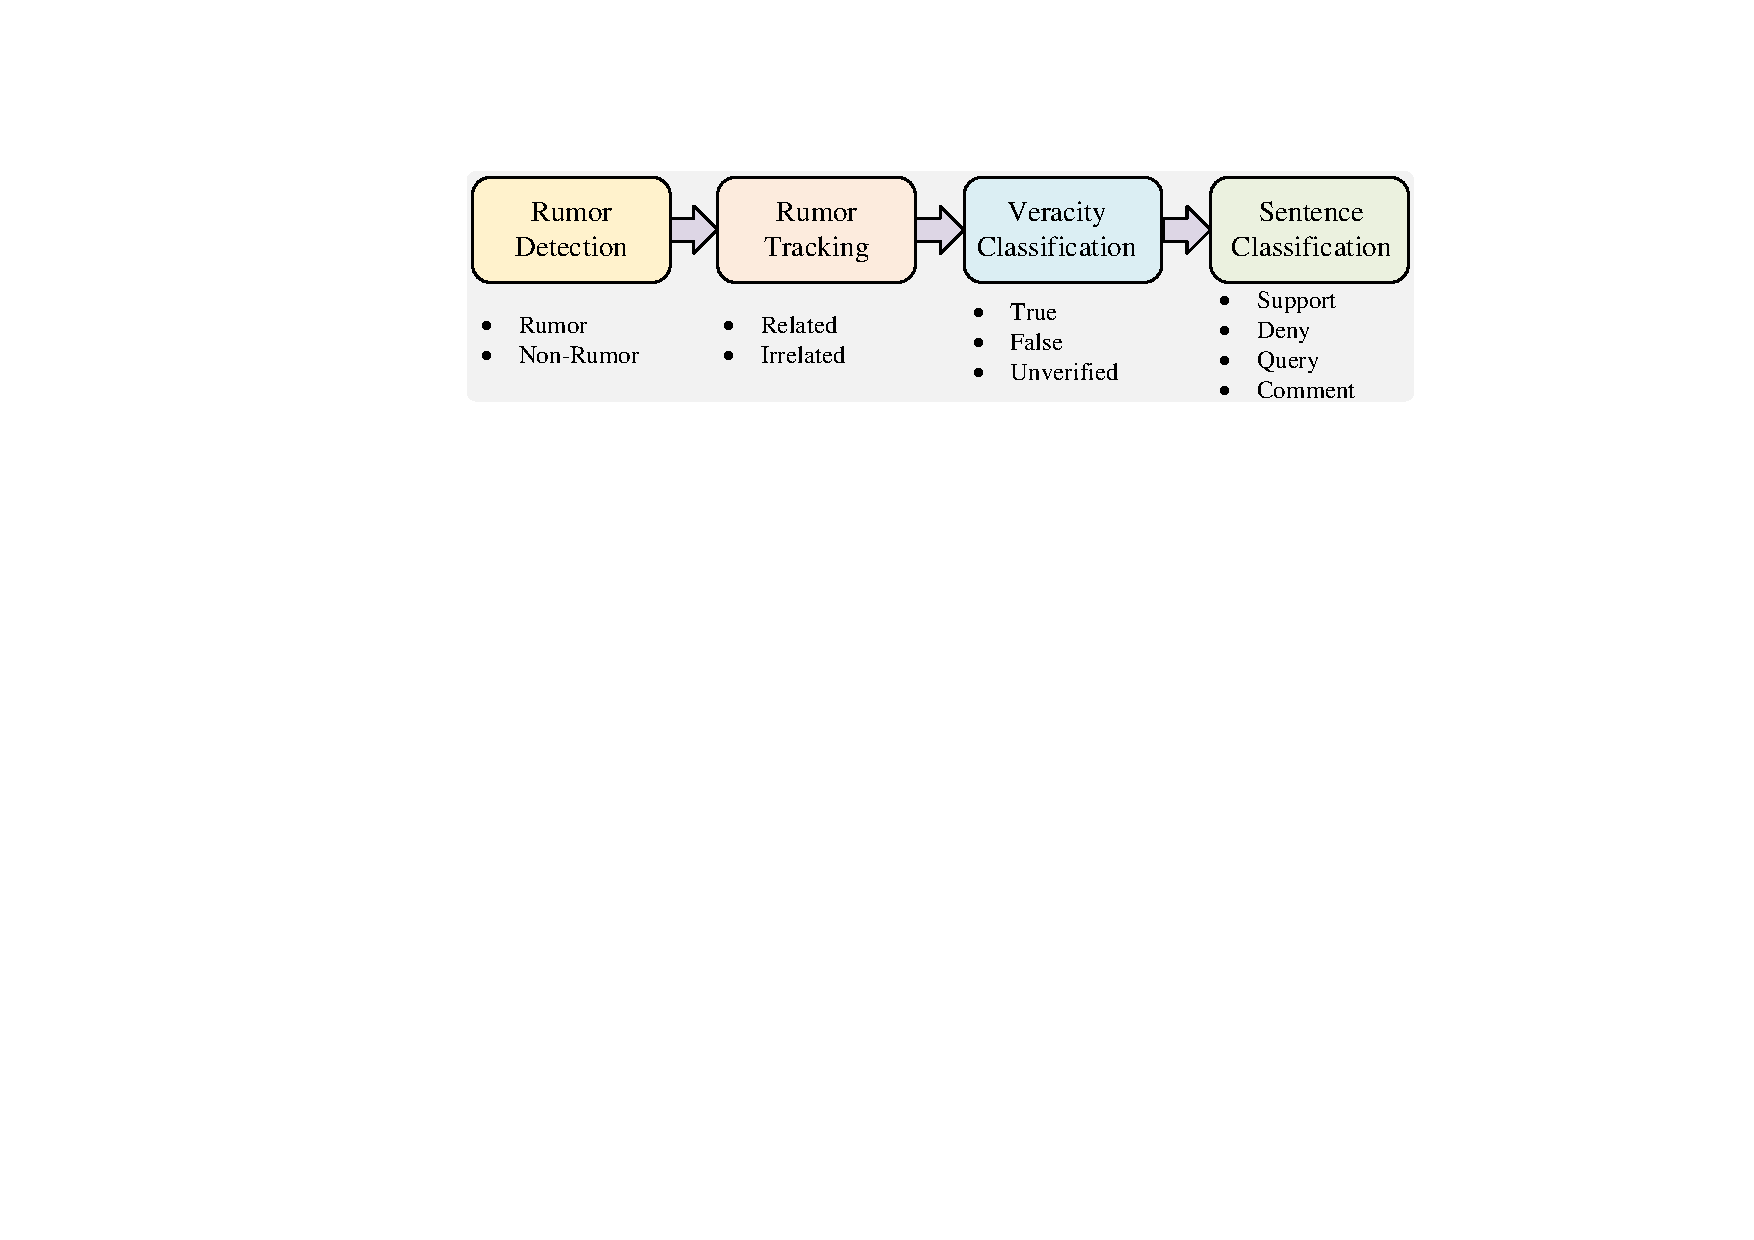
\includegraphics[width = \textwidth]{fig/pipeline}
	\caption{Pipeline of Rumor Detection Task}
	\label{fig:pipeline}
\end{figure}
\section{Preliminaries}
\label{sec:perliminary}

\begin{figure}[tbp]
	\hspace{0ex}
	\vspace{0ex}
	\centering
	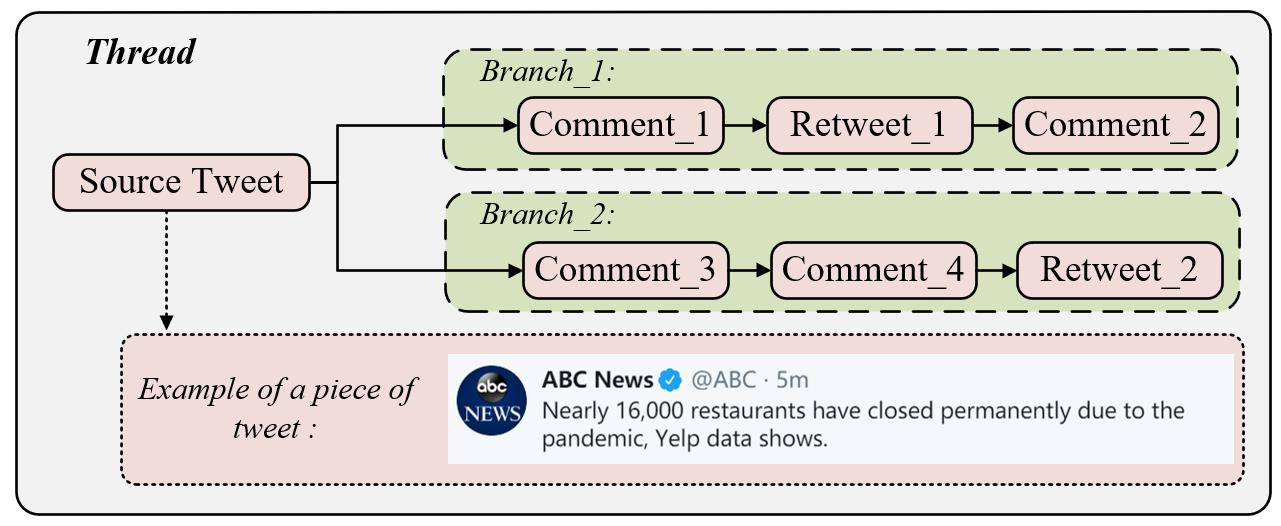
\includegraphics[width = \textwidth]{fig/data_format}
	\caption{The data format of a tweet thread}
	\label{fig:data_format}
\end{figure}

In this section, we proceed to introduce the notations, problem definitions, and background knowledge of rumor tracking. The frequently used notations are summarized in Table~\ref{tab:notations}.

\subsection{Social Network Data}
\label{sec:social_network_data}
We use two benchmark datasets PHEME \cite{DBLP:conf/coling/KochkinaLZ18} and RumorEval \cite{DBLP:conf/semeval/EnayetE17}. Each dataset is a set of rumor events and each event is a set of tweet threads. The data format of a tweet thread is shown in Fig.~\ref{fig:data_format}. Each tweet thread is a tree structure. The root node corresponds to source tweet and the branches correspond to a tweet sequences that includes retweets and comments. A tweet contains various types of features, including content, publication time, screen name, etc. The statistical details of PHEME and RumorEval are shown in Table \ref{tab:pheme} and Table \ref{tab:RumorEval}, respectively.

\begin{table}[tbp]
	\caption{Notation Summarization}
	\centering
	\label{tab:notations}
	\resizebox{0.55\linewidth}{!}{
	\begin{tabular}{|c|l|}
		\hline
		\textbf{Notation} & \textbf{Definition}\\
		\hline
		$T$ & the set of tweets \\
		\hline
		$y_F'$ & output of FastText \\
		\hline
		$t_n$ & a tweet\\
		\hline		
		$y_T'$ & output of TextCNN\\
		\hline
		$C$ & the set of rumor events\\
		\hline
		$y_B'$ & output of BiLSTM\\
		\hline
		$c_m$ & a rumor event \\
		\hline
		$y_N'$ & output of Naive Bayes\\
		\hline
		$r$ & predictable result of a component\\
		\hline
		$y_S'$ & output of SGD\\
		\hline
		$R$ & predictable result of ART\\
		\hline
		$y'$& output of ART\\
		\hline
		$x \in R^{l*d}$ & a processed sample\\
		\hline
		$y \in R^m$ & a training label\\
		\hline
		$K_y$ & set of all components outputs\\		
		\hline						
	\end{tabular}
	}
\end{table}

\subsection{Problem Definition}
\label{sec:problem}
Let $T = \left\{t_1, t_2, ..., t_n \right\}$ denote a set of tweets and each tweet is denoted as $t_n$. Let $C = \left\{c_1, c_2, ... , c_m \right\}$ denote a set of rumor events and $c_m$ denotes a particular rumor event. Each tweet is assigned to only one rumor event. For each given tweet $t_n$, the goal of rumor tracking is to find the most relevant rumor event. In this work, we transform the binary rumor tracking problem (relevant/irrelevant) into an m-way classification problem. 

We conduct a preprocessing procedure to embed the $T$ and $C$ into vectors. In preprocessing, a tweet $t_n \in T $ is padded to a fixed length $l$. Then, each word in the $l$-length tweet $t_n$ is embedded to a d-dimensional vector so that $t_n$ is transformed to a tensor $x^{(i)} \in R^{l*d}$. Also, we embed each event $c_m \in C$ to a one-hot vector $y^{(i)} \in R^m$. By preprocessing, the dataset is transformed into: $$\left\{ (x^{(1)}, y^{(1)}), (x^{(2)}, y^{(2)}),..., (x^{(n)}, y^{(n)}) \right\}, x^{(i)} \in R^{l*d}, y^{(i)} \in R^m $$ The goal is transformed to predicting the $y^{(i)}$ for a given $x^{(i)}$. Existing work \cite{DBLP:conf/www/ChengNB20} links a testing sample $x^{(i)}$ with its source tweet. This setting disturbs the fairness of classification when predicting. In this work, we ensure that the branch and thread of a testing sample $x^{(i)}$ is unknown when predicting.

In a rumor event, the source tweets are collected by keywords such that the semantic similarity between the source tweets is usually high. We observe that this high similarity between the source tweets disturbs the classification performance. To verify our assumption, we conduct an experiment to train a rumor event classifier by using source tweets as input. The classification result suggests that the accuracy even reaches 100\%. Consequently, we cut down the link between tweet and its source, and then process each tweet independently to obtain a convincing result. 

\subsection{Basic Models for Text Classification}
\label{sec:deeplearning_model} 
In this section, we proceed to introduce some basic text classification models.

\subsubsection{Non-Deep Learning based Models}
\textbf{Naive Bayes} \cite{DBLP:journals/ml/DomingosP97} is widely adopted for short text classification which shows good performance. It assumes that all input variables are independent of each other. By multiplying the conditional probabilities of each word, it achieves satisfied performances on text classification task with only small quantities of parameters. The procedure of Naive Bayes is formalized as follows:
\begin{align}\label{eq:nb}
y_{N_{i}}' &= \frac{P(y_i)\prod_{j = 0}^d P(x_j|y_i)}{\prod_{j = 0}^d P(x_j)},\\
y_N' &= concat(y_{N_{1}}',y_{N_{2}}',..., y_{N_{i}}'),
\end{align}
where $x_j$ is a component of $x$, corresponding to a word in tweet.  $y_i$ is a component of training sample $y$. $y_{N_{i}}'$ is a component of $y_N'$, representing the probability of a classification. We choose Naive Bayes as  a component of ART and  $y_N'$ is the final output.

\textbf{SGD} \cite{avriel2003nonlinear} is a parameter updating policy in machine learning, which is widely adopted in text classification with large-scaled corpus. SGD based machine learning models are trained on large scale datasets by updating parameters on each single sample. We denote the procedure of SGD model as $S()$, and the output of SGD model is:
\begin{equation}\label{eq:sgd}
y_S' = S(TFIDF(x)),
\end{equation}
where TFIDF is Term Frequency-Inverse Document Frequency. Finally, we choose SGD based classification model as the component of ART.

\subsubsection{Deep Learning based Models}

\textbf{FastText} \cite{DBLP:journals/tacl/BojanowskiGJM17, DBLP:journals/corr/JoulinGBDJM16, DBLP:conf/eacl/GraveMJB17} is an extension of the skip-gram model introduced by Mikolov et al. \cite{DBLP:conf/nips/MikolovSCCD13}. The main difference between FastText and skip-gram is that the predictable target of FastText is a classification label rather than a middle word. Also, FastText adopts hierarchical softmax to deal with the large corpus and vocabulary dictionary. With the help of these optimizations, FastText classifies large amounts of texts in a short time. We choose FastText as a component of ART and its output is denote as $y_F'$.

\textbf{BiLSTM} \cite{DBLP:journals/neco/HochreiterS97} is Bi-directional Long Short-Term Memory, which is consisted of a forward-LSTM and a backward-LSTM. BiLSTM effectively learns the long term dependency of sequential data. So we usually treat it as a evolution of LSTM and it is suitable for text data. The details of BiLSTM are following:
\begin{align}\label{eq:lstm}
x_tL/R &= Embedding(x_tL/R), \\
x_t &= concat(x_tL, x_tR), \\
i_t &= \sigma(W_i \cdot [h_{t-1}, x_t] + b_i),\\
f_t &= \sigma(W_f \cdot [h_{t-1}, x_t]),\\
\widetilde{C_t} &= tanh(W_{\tilde{C_t}} \cdot [r_t C_{t-1}, x_t]  + b_C),\\
C_t &= (1-f_t) C_{t-1} + f_t \widetilde{C_t},\\
h_t &=o_t \* \tanh(C_t),\\
y_B^{'} &= o_t =  \sigma(W_o \cdot h_t),
\end{align}
where $x_t$ is the input at time step $t$, and it is concatenated by leftward unit $x_tL$ and rightward unit $x_tR$. BiLSTM consists of three gates: forget gate $f_t$, input gate $i_t$, and output gate $o_t$. Also, it has two memories: long-term memory $C_t$ and short-memory $h_t$. Finally, we use output $o_t$ as the final output of BiLSTM, which is denoted as $y_B^{'}$.

\textbf{TextCNN} \cite{DBLP:conf/emnlp/Kim14} uses multiple convolutional filters with different sizes to capture N-gram features. Compared to RNN based models, TextCNN reaches convergence faster due to the parallel computation. The tweets are usually short text (within 140 words) with sparse semantic. Consequently, CNN based models are more suitable than RNN based models for tweets classification because tweets are usually treated as a bag of words. We choose TextCNN as one of the components of ART. The brief procedure of TextCNN is shown as follows,

\begin{align}\label{eq:tcnn}
V_x &= Embedding(x), \\
m_3 &= maxpooling(ConV_3(V_x)),\\
m_4 &= maxpooling(ConV_4(V_x)),\\
m_5 &= maxpooling(ConV_5(V_x)),\\
y_T' &= flatten(concat(m_3, m_4, m_5)),
\end{align}
where the $Embedding()$ is the embedding layer, and $m$ is the output of different convolutional filter. By concatenating and flattening, TextCNN generates the output that is denoted as $y_T'$.
\section{\textcolor{blue}{Deep Reinforcement Learning based Ensemble Model for Rumor Tracking}}
\label{sec:model}

\textcolor{blue}{RL-BRT model is inspired by Mixture of Experts model (MoE) \cite{DBLP:conf/nips/MillerU96}. MoE is an ensemble model that contains multiple separate sub-models. Each sub-model is an expert that is trained on a region of input data. The data distribution of each tweet is different and we believe each rumor tweet has its suitable classifier. Therefore, instead of dividing the input data into different regions, RL-ERT adopts a policy gradient based neural network to generate a weight for each sub-model and then aggregates them together. Besides, the weight changes according to each input sample.}

Ensemble model \cite{DBLP:journals/ml/Breiman96b} aggregates different basic models as its components. With a proper ensemble strategy, the performance is usually better than that of the basic models. Ensemble model reduces variance and improves the
stability of estimated density. Besides, the multiple components balance each other to reduce overfitting. Also, the most suitable classifier for different types of features is changing, and therefore multiple components are more likely to contain the proper classifier. Moreover, the importance of components changes according to the samples. Therefore, we propose a reinforcement learning based weight-tuning policy network (WTPN) to generate a suitable weight to balance the importance of components for each sample. 

\subsection{Architecture}
\label{sec:architecture}
The architecture of \textcolor{blue}{RL-ERT} is shown in Fig.~\ref{fig:architecture} . The input of \textcolor{blue}{RL-ERT} consists of two types of features, which include content features and social features. Then, all features are embedded and sent to basic components.  Some components such as TextCNN and BiLSTM use word-to-vector embeddings and the other components use particular embedding methods. Next, each trained component makes its prediction separately. Finally, we add the predicted results of all components and generate a final prediction by a reinforcement learning based ensemble algorithm.

\subsection{Preprocessing and Embedding}
\label{sec:process_embedding}
The textual content is one of the most important features in rumor tracking task. The length of the textual content is short, which is restricted within 140 words. Usually, the spelling in tweets is causal with symbols mixed in it. Consequently, we clean the content before inputting them into the model. The preprocessing in NLP is roughly immobilized, we only make some minor adjustments. In this work, we adopt splitting on tweets, and then remove the punctuation and special characters. Next, we turn all characters into lowercase. Finally, we adopt lemmatization on all words.

We find that the embedding strategies have a significant impact on the performance of \textcolor{blue}{RL-ERT}. Therefore, we try different embedding strategies to find the most proper one. There are three commonly used embedding strategies: pre-trained embedding, self-trained embedding, and random embedding. Pre-trained embedding is trained on large-scale corpus, and the most representative ones are GloVe \cite{DBLP:conf/emnlp/PenningtonSM14} and Google News embedding \cite{googlenews}. The self-train embedding is to train embedding on the current dataset. And the random embedding is to assign each word to a unique embedding randomly. In this work, we try all three embedding strategies and the detailed performance is introduced in Section \ref{sec:experiment}. By comparing them, we finally choose random embedding as the embedding strategy in \textcolor{blue}{RL-ERT}.

\begin{algorithm}[tbp]
	\caption{Ensemble Algorithm}
	\label{algorithm:RL-BRT}
	\LinesNumbered % show line numbers
	\KwIn{$K_y = \left\{y_F', y_T', y_B', y_N', y_S' \right\}$: outputs of all components;
		$x \in R^{l \times d}$: a processed sample;
		$WTPN$: weight-tuning policy network}
	\KwOut{$R$: predicted result of \textcolor{blue}{RL-ERT};}
	\textbf{Initialize:} Outputs of \textcolor{blue}{RL-ERT}: $y' = [0]*m$, $R = 0$ \;
	$W_y =  WTPN(x, K_y)$ \;
	\For{$i$ in $\{F,T,B,N,S\}$}{
		$y'+= w_i \cdot y_i'$;
	}
	
	$R = argmax(y')$
\end{algorithm}

\subsection{Procedure of \textcolor{blue}{RL-ERT}}
As shown in Fig.~\ref{fig:architecture}, we make preprocessing on \textbf{content features}. Despite some content features, the tweets contain plenty of \textbf{social features}. As introduced in Section \ref{sec:problem}, the tweet's branch or thread is unknown in advance. Consequently, we omit some features that contain external information about the branch or thread. Finally, we choose ``screen name", ``reply to screen name", and ``hashtag" as the social features in \textcolor{blue}{RL-ERT}. We treat the social features as words and add them to the tweets, then concatenate the content features and social features. All components are trained respectively until getting convergence. When predicting, each component outputs an $m-$dimensional vector $y'$ after the softmax layer. Each component in $y'$ indicates the probability of the content belongs to this category. 

With all components in \textcolor{blue}{RL-ERT} trained, we aggregate them and make a final prediction on the rumor tracking task. Generally, frequently used bagging methods include \textbf{joint training} and \textbf{respective training}. Joint training means all models have one shared loss function, and all parameters are updated together. When predicting, the ensemble model directly outputs the final prediction. Respective training means we train each component respectively. When predicting, each component makes its prediction result. In \textcolor{blue}{RL-ERT}, we choose the respective training. 

As all components are trained, results are aggregated by an ensemble algorithm. The ensemble details of \textcolor{blue}{RL-ERT} are shown in Algorithm~\ref{algorithm:RL-BRT}. We denote the predicted result of \textcolor{blue}{RL-ERT} as $R$. The inputs of Algorithm~\ref{algorithm:RL-BRT} are a sample $x$ and its predicted results of all components, which are denoted as $K_y = \left\{y_F', y_T', y_B', y_N', y_S' \right\}$. Each element in $K_y$ is an $m-$dimensional vector. Then, $x$ and $K_y$ is sent to WTPN and the output is a set of weights denoted as $W_y$ (Line 2). Each element $y_i'$ in $K_y$ is assigned with a weight in $W_y$. Next, we sum the predicted results in $K_y$ with weights (Line 4). Finally, the category with the maximum possibility is the predicted result of \textcolor{blue}{RL-ERT} (Line 6). 

\begin{figure}[tbp]
	\hspace{0ex}
	\vspace{0ex}
	\centering
	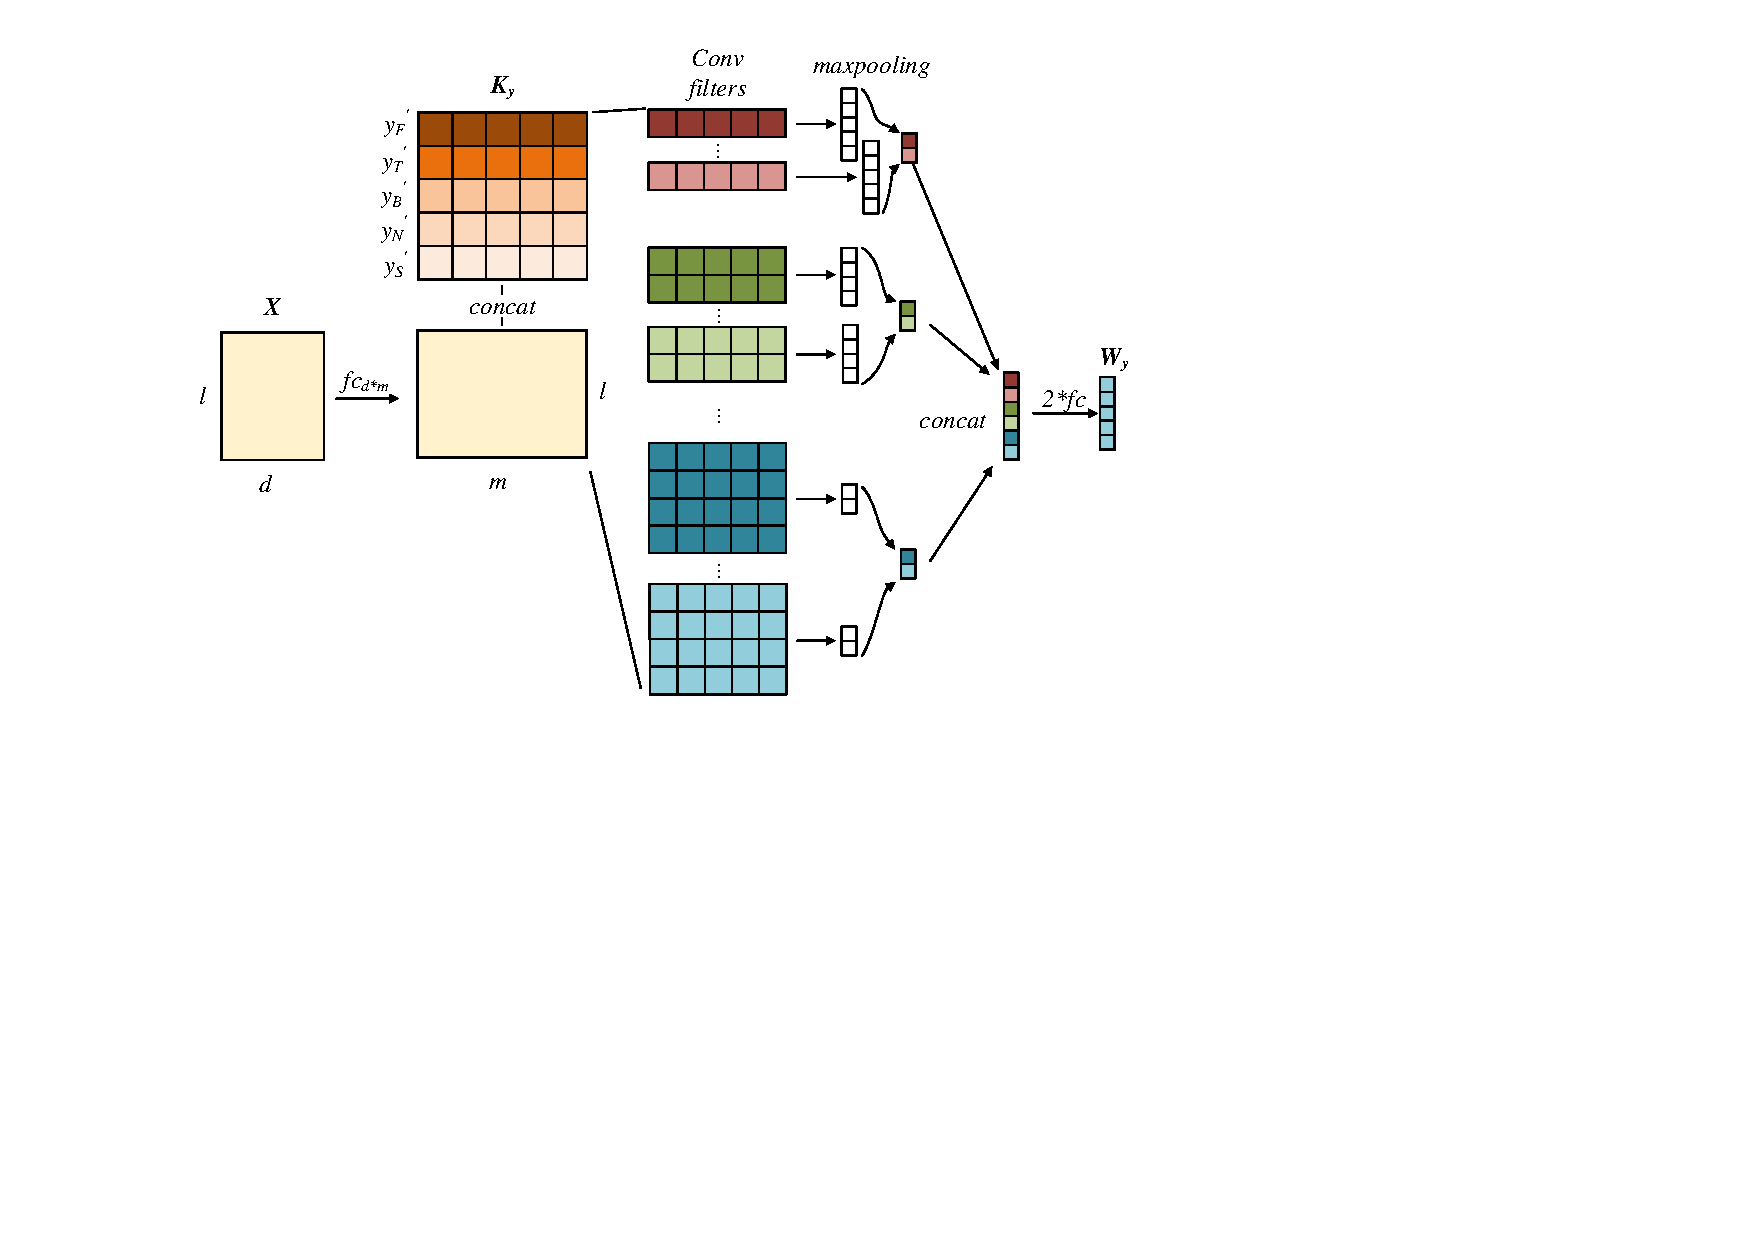
\includegraphics[width = \textwidth]{fig/WTPN}
	\caption{Structure of WTPN}
	\label{fig:WTPN}
\end{figure}

\subsection{Weight-Tuning Policy Network}
We propose WTPN to generate a suitable weight for each sample. WTPN is based on a reinforcement learning structure with a triple-tuple $<S, A, R>$, where $S = \{ s \}$ is a set of states. $A = \{ a \}$ is a set of actions. $R(s, a)$ is the reward function.
\begin{itemize}
	\item \textbf{State} $s$: $s = ( x, K_y )$ denotes a state of WTPN, where $x$ is a sample and $K_y$ is the set of classification results of $x$ generated by different classifiers.
	
	\item \textbf{Action} $a$: $a = W_y$ denotes a set of weights corresponding to elements in $K_y$.
	
	\item \textbf{Reward} $R$: $R(s, a) \to r \in R^{S * A}$ is a reward function that measures the profit of the current state-action tuple $(s, a)$.
\end{itemize}

For a batch of samples $X_b$, the accumulated reward is defined as:
\begin{equation}
R(s_1, a_1, ..., s_{|X_b|},a_{|X_b|}) = \frac{1}{|X_b|}\sum_{t = 1}^{t = |X_b|} r_t,
\end{equation}
where $ \frac{1}{|X_b|}$ is a normalization item. For a sample, $R(s,a) = r$ is the negative softmax cross-entropy loss between the predicted result (Line 6 in Algorithm \ref{algorithm:RL-BRT}) and ground-truth label.
For each batch, the parameter $\theta$ of policy function is updated by the following equation: 

\begin{align}
\theta &\leftarrow \theta + \lambda \nabla_\theta J_b(\mu_\theta),\\
J_b(\mu_\theta) &= \mathbb{E} [R(s_1, a_1, ..., s_{|X_b|},a_{|X_b|}) ],
\end{align}
where $\lambda$ is learning rate. $J_b(\mu_\theta)$ is the expected return.
The goal of WTPN is to approximate a policy function $\mu_\theta :S \to A$ that maximizes the accumulated reward.  Inspired by \cite{DBLP:conf/aaai/KimJSR16}, we propose a CNN based WTPN structure. As shown in Fig.~\ref{fig:WTPN}, the inputs of WTPN are $x$ and $K_y$, and the output is $W_y$. $x$ is sent to an FC (full-connect) layer and concatenated with $K_y$. We adopt multiple filters on the concatenated vector. The sizes of multiple filters are different, including  $[2*m]$, $[3*m]$, $[4*m]$, and $[5*m]$. The convolutional padding strategy is the same. By convolution and max-pooling, WTPN concatenates the captured features. Finally, with 2 FC layers, WTPN outputs $W_y$. \textcolor{blue}{In WTPN, we concatenate two separate inputs to a sequence. Then we use filters of different sizes to capture the features in different scales. Finally, we use max-pooling to reduce the model size and remove the unimportant parameters. The structure of WTPN is similar to TextCNN because TextCNN is an effective feature extractor, which is suitable to address the sequential data. Besides, the CNN based structure is calculated in parallel easily and is very efficient. Finally, we build a CNN based structure as shown in Fig.\ref{fig:WTPN}.}
\section{Experiment}
\label{sec:experiment}
In this section, we proceed to introduce the experimental settings and results. Our GPU device is Tesla P100 with 16GB memory. We use python 3.7 based Keras to implement all the experiments.

\subsection{Datasets and Baselines}
\label{sec:dataset}
The datasets of our experiment are  PHEME \cite{DBLP:conf/coling/KochkinaLZ18} and RumorEval \cite{DBLP:conf/semeval/EnayetE17}. These two datasets are widely used in the rumor detection research area. The details of PHEME are shown in Table.\ref{tab:pheme} and the details of RumorEval are shown in Table.\ref{tab:RumorEval}. The original PHEME contains 9 events and 4 of them are sparse, so we usually use PHEME-5 (following the existing works \cite{DBLP:conf/www/ChengNB20}). The PHEME-5 is formed by the top-5 scaled events, which contains 5802 threads and 1972 in them are rumors. 

To demonstrate the effectiveness of ART, we choose baselines as comparisons, including (Naive Bayes, SGD, Dense, BiLSTM) \cite{DBLP:conf/emnlp/QazvinianRRM11}, FastText\cite{DBLP:conf/eacl/GraveMJB17}, TextCNN\cite{DBLP:conf/emnlp/Kim14}, VRoC \cite{DBLP:conf/www/ChengNB20}, and some combinations of them. All the chosen baselines are contained in Table.\ref{tab:results_RE}. We use accuracy and micro-F1 as the evaluation metrics.

\begin{table}[htbp]
	\caption{PHEME}
	\centering
	\label{tab:pheme}
	\resizebox{0.8\linewidth}{!}{
		\begin{tabular}{|c|c|c|c|}
			\hline
			\textbf{Events} & \textbf{Threads} & \textbf{Tweets} & \textbf{Threads of Rumors}\\
			\hline
			Charlie Hebdo &2079&38268&458\\
			\hline
			Sydney siege  &1221&23996&522\\
			\hline
			Ferguson &1143&24175&284\\
			\hline
			Ottawa Shooting &890&12284&470\\
			\hline		
			Germanwings-crash&469&4489&238\\
			\hline
			\textbf{Total} & 5802 & 103212 & 1972 \\
			\hline	
		\end{tabular}
	}	
\end{table}

\begin{table}[htbp]
	\caption{RumorEval}
	\centering
	\label{tab:RumorEval}
	\resizebox{0.6\linewidth}{!}{
		\begin{tabular}{|c|c|c|c|}
			\hline
			\textbf{}  & \textbf{Threads} & \textbf{Branch} & \textbf{Tweets}\\
			\hline
			Development  &25&215&281\\
			\hline
			Testing  &28&772&1049\\
			\hline
			Training &272&3030&4238\\
			\hline	
			\textbf{Total}  &325 &4017 &5568 \\
			\hline		
		\end{tabular}
	}	
\end{table}


\subsection{Experimental Results}
The results on RumorEval are shown in Table.~{\ref{tab:RumorEval}}. The second column records the F1-Scores on each event, and "F, O, S, C, G" are the first chars of the corresponding event name. The results suggest that ART achieves the best performance on both average accuracy and average F1-Score. TextCNN gets the best performance among these basic models. It is because the bag-of-words idea in TextCNN is suitable for the short text and various filters with different length effectively capture the features of key grams. Naive Bayes gets the worst performance. We think the reason is that the parameters in Naive Bayes are limited, which is not enough for this corpus. SGD+TextCNN achieves the best performance among the pairwise-added models. 

The results on PHEME are shown in Table.~\ref{tab:results_PHE}. It suggests that ART model gets the second-best performance on average accuracy and average Micro-F1 score, which is a little lower than the combination of FastText, Dense, and TextCNN. We think it is because the scale of PHEME is larger than that of the RumorEval, and the SGD is not suitable for large-scaled dataset. Consequently, the worse performance of SGD affects the performance of ART. Also, the performance of basic models on PHEME proofs our explanation. The SGD gets the worst performance among all basic models. For F1-Score on every event, ART gets the best performance on two events, which ties the performance of the combination of FastText, Dense, and TextCNN. To sum up, ART gets satisfactory performance on all datasets, which proved
the effectiveness.

\begin{table}[htbp]
	\caption{Results on RumorEval}
	\centering
	\label{tab:results_RE}
	\resizebox{1\linewidth}{!}{
		\begin{tabular}{|c|c|c|c|}
			\hline
			\multirow{2}{*}{\textbf{Methods}}  & \textbf{F1-Score on each event} & \multirow{2}{*}{\textbf{Average Accuracy}} & \multirow{2}{*}{\textbf{Average Micro-F1}}\\
			& \textbf{F/ O/ S/ C/ G} &  & \\
			\hline
			NB  & 0.937/0.924/0.907/0.929/0.617 & 0.910 & 0.863\\
			\hline
			SGD  & 0.977/0.964/0.942/0.928/0.927 & 0.950 & 0.948\\
			\hline
			FastText & 0.973/0.944/0.927/0.905/0.954
			& 0.938 & 0.940 \\
			\hline	
			Dense  & 0.964/0.951/0.939/0.937/0.919
			&0.946 &0.942 \\
			\hline
			BiLSTM  & 0.972/0.909/0.910/0.895/0.901
			&0.920 &0.917 \\
			\hline
			TextCNN  & 0.991/\textbf{0.964}/0.939/0.934/0.900
			& 0.953 & 0.946 \\
			\hline
			FastText + Dense  &0.979/0.951/0.936/0.918/0.964
			& 0.947 & 0.950 \\
			\hline
			FastText + TextCNN  & 0.975/0.940/0.925/0.898/0.954
			& 0.935 & 0.938 \\
			\hline
			SGD + TextCNN  & 0.979/0.964/0.942/0.935/0.927
			& 0.953 & 0.950 \\
			\hline
			Dense + TextCNN  & 0.964/0.954/0.945/0.926/0.88
			& 0.942 & 0.934 \\
			\hline
			FastText+ Dense + TextCNN  & 0.979/0.947/0.932/0.907/\textbf{0.964}
			& 0.942 & 0.946 \\
			\hline
			FastText+ SGD + TextCNN  & 0.977/0.955/0.941/0.925/0.937
			& 0.948 & 0.947 \\
			\hline
			VRoC  &0.640/0.703/0.611/0.685/0.520
			& 0.644 & 0.632 \\
			\hline
			ART  & \textbf{0.979}/0.961/\textbf{0.952}/\textbf{0.943}/0.937
			& \textbf{0.956} & \textbf{0.955} \\
			\hline					
		\end{tabular}
	}	
\end{table}

\begin{table}[htbp]
	\caption{Results on PHEME}
	\centering
	\label{tab:results_PHE}
	\resizebox{1\linewidth}{!}{
		\begin{tabular}{|c|c|c|c|}
			\hline
			\multirow{2}{*}{\textbf{Methods}}  & \textbf{F1-Score on each event} & \multirow{2}{*}{\textbf{Average Accuracy}} & \multirow{2}{*}{\textbf{Average Micro-F1}}\\
			& \textbf{F/ O/ S/ C/ G} &  & \\
			\hline
			NB  & 0.976/0.926/0.888/0.900/0.735
			& 0.907 & 0.885\\
			\hline
			SGD  & 0.964/0.897/0.875/0.884/0.880
			&0.893&0.880\\
			\hline
			FastText &0.980/0.922/0.915/0.902/0.919
			&0.927&0.927\\
			\hline	
			Dense  & 0.977/0.912/0.905/0.891/0.913
			& 0.919 & 0.920 \\
			\hline
			BiLSTM  & 0.978/0.931/0.909/0.899/0.932
			& 0.927 & 0.930 \\
			\hline
			TextCNN  & 0.984/0.927/0.919/0.901/0.917
			& 0.930 & 0.930 \\
			\hline
			FastText + Dense  & 0.981/0.924/0.916/0.903/0.916
			& 0.928 & 0.928 \\
			\hline
			FastText + TextCNN  &0.984/0.928/0.923/0.910/0.927
			& 0.934 & 0.934 \\
			\hline
			SGD + FastText  & 0.981/0.925/0.913/0.904/0.913
			& 0.927 & 0.927 \\
			\hline
			Dense + TextCNN  & 0.986/0.894/\textbf{0.926}/0.908/0.930
			& 0.927 & 0.929 \\
			\hline
			FastText+ Dense + TextCNN  &0.987/0.935/0.925/\textbf{0.918}/ \textbf{0.930}
			& \textbf{ 0.939} & \textbf{0.939} \\
			\hline
			FastText+ SGD + TextCNN  & 0.982/0.932/0.922/0.912/0.926
			& 0.934 & 0.935 \\
			\hline
			ART  &\textbf{0.988}/\textbf{0.937}/0.921/0.915/0.917
			& 0.936 & 0.935 \\
			\hline					
		\end{tabular}
	}	
\end{table}

\subsection{Different Embedding Strategies}
As introduced in Section~\ref{sec:process_embedding}, there are three embedding strategies. To find the most proper embedding strategy, we conduct experiments on three representative basic models including Dense, BiLSTM, and TextCNN. The experimental results are shown in Table.~\ref{tab:embedding}. We find that the random embedding strategy significantly outperforms the others on both average accuracy and average micro-F1. Self-trained embedding strategy achieves the second-best performance with a little superiority than that of the Google News Word2Vector. Moreover, we also test the GloVe embedding and the results are worse than Google News Word2Vector. The existing work usually adopts the pre-trained embedding strategy. However, we find that the most proper embedding strategies are random embedding. Therefore we choose random embedding in the ART.

\begin{table}[htbp]
	\caption{Results of Different Embedding Strategies}
	\centering
	\label{tab:embedding}
	\resizebox{0.9\linewidth}{!}{
		\begin{tabular}{|c|c|c|c|}
			\hline
			\multirow{2}{*}{Events}  & \textbf{F1-Score on each event} & \multirow{2}{*}{\textbf{Average Accuracy}} & \multirow{2}{*}{\textbf{Average Micro-F1}}\\
			& \textbf{F/ O/ S/ C/ G} &  & \\
			\hline
			\multicolumn{4}{|c|}{\textbf{Google News Word2Vector}} \\
			\hline
			Dense  & 0.651/0.440/0.547/0.467/0.400
			& 0.542 & 0.501\\
			\hline
			BiLSTM  & 0.771/0.584/0.697/0.681/0.576
			&0.675&0.662\\
			\hline
			TextCNN  & 0.760/0.594/0.735/0.710/0.538
			& 0.689 & 0.667 \\
			\hline
			\multicolumn{4}{|c|}{\textbf{Self-trained Word2Vector}} \\
			\hline
			Dense  & 0.727/0.532/0.629/0.620/0.575
			& 0.635 & 0.616\\
			\hline
			BiLSTM  & 0.907/0.739/0.789/0.792/0.694
			&0.806&0.784\\
			\hline
			TextCNN  & 0.812/0.678/0.776/0.766/0.618
			& 0.757 & 0.730 \\
			\hline	
			\multicolumn{4}{|c|}{\textbf{Random Embedding}} \\
			\hline
			Dense  & 0.964/0.951/0.939/0.937/0.919
			& \textbf{0.946} &\textbf{0.942} \\
			\hline
			BiLSTM  & 0.972/0.909/0.910/0.895/0.901
			&\textbf{0.920} &\textbf{0.917} \\
			\hline	
			TextCNN  & 0.991/0.964/0.939/0.934/0.900
			& \textbf{0.953} & \textbf{0.946} \\
			\hline	
		\end{tabular}
	}	
\end{table}

\begin{figure}[tbp]
	\centering
	\subfigure{
		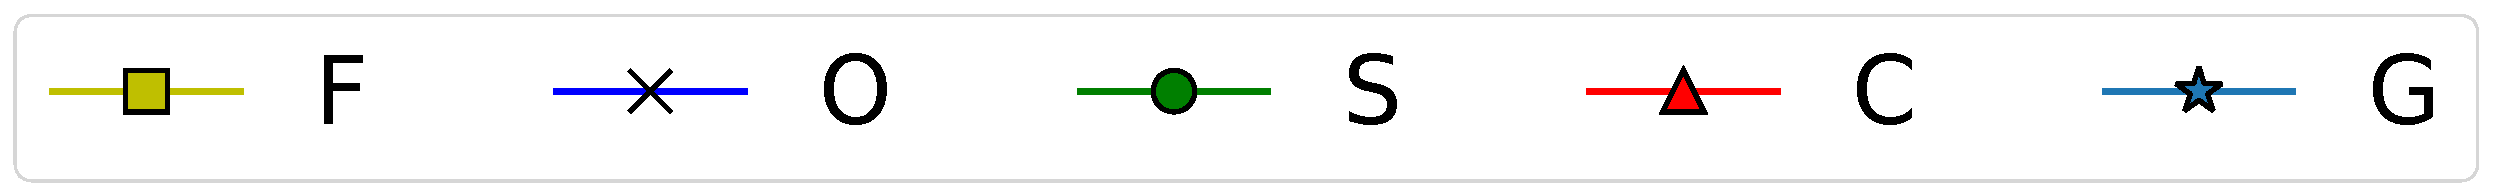
\includegraphics[width=0.4\linewidth]{fig/legend_f1}
	}
	\setcounter{subfigure}{0}
	\subfigure[Affects of Parameters on Different Events]{
		\label{fig:parameter_events}
		\begin{minipage}[b]{0.35\linewidth}
			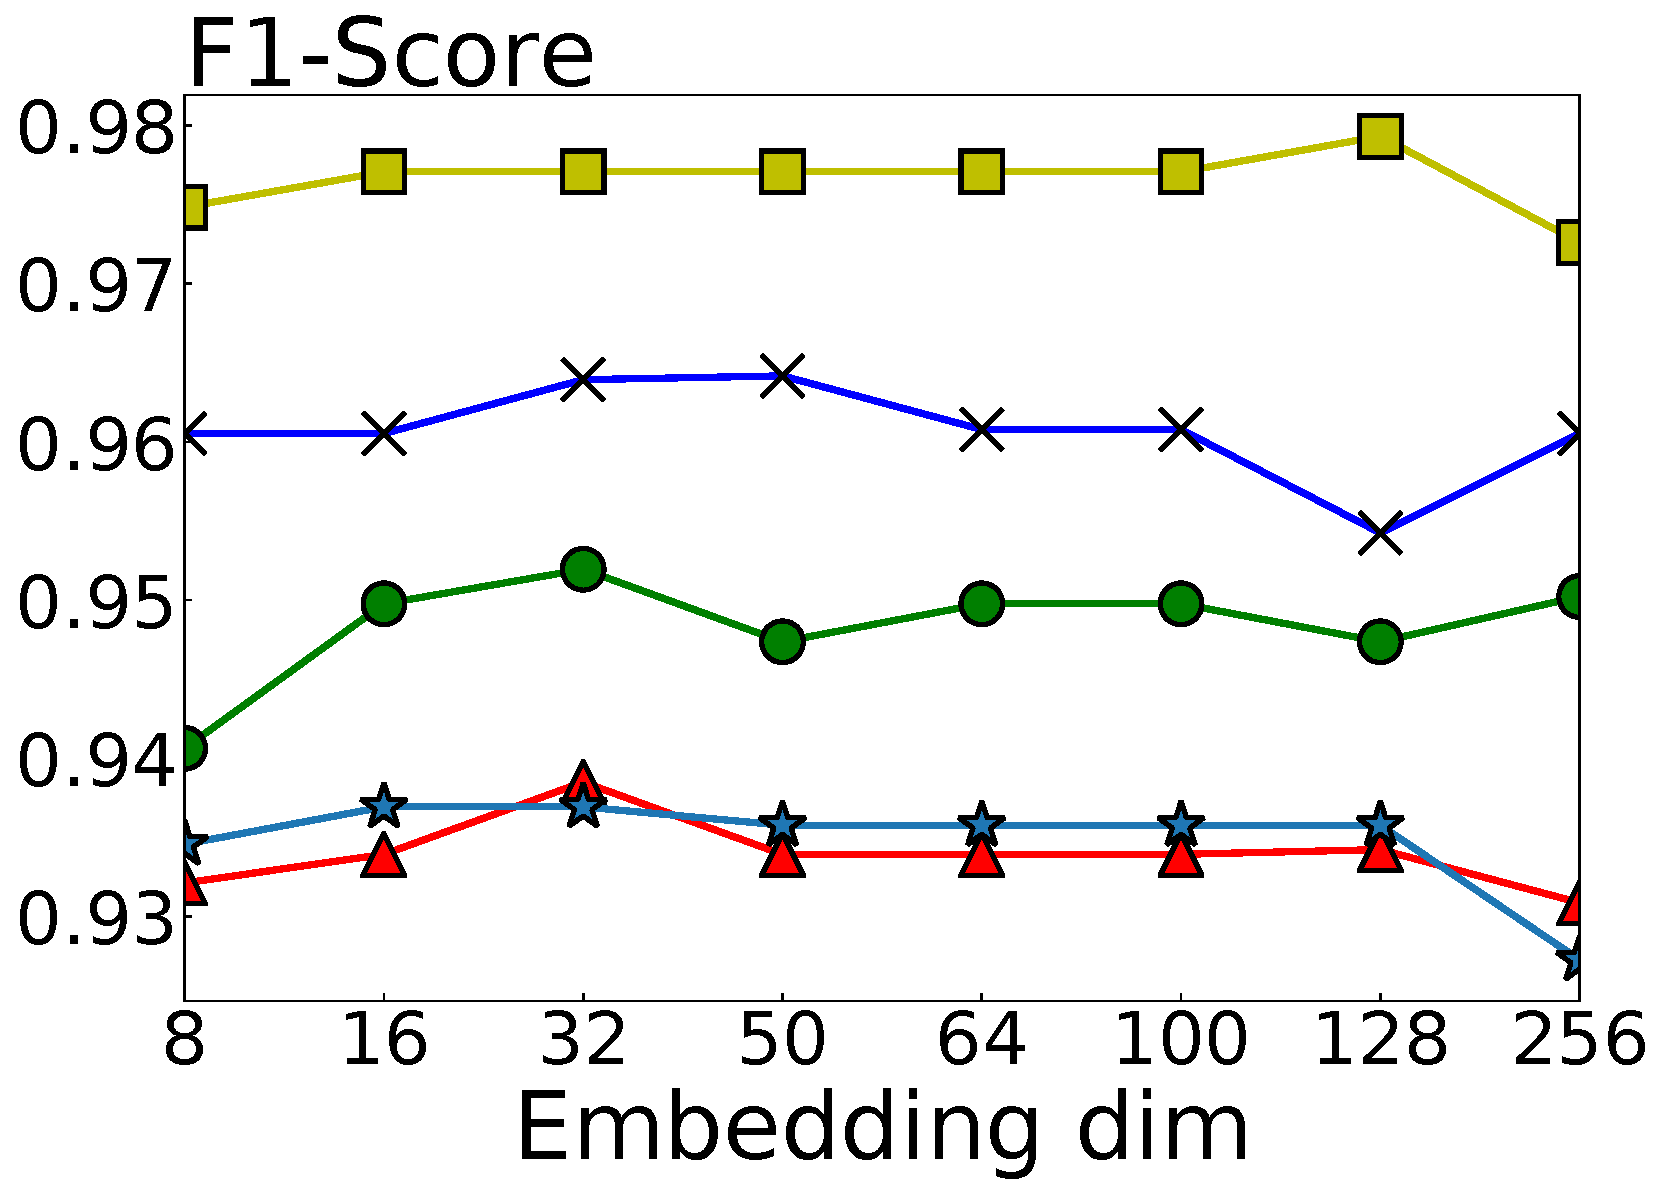
\includegraphics[width=1\linewidth]{fig/embedding_dim_events}
		\end{minipage}
		\begin{minipage}[b]{0.35\linewidth}
			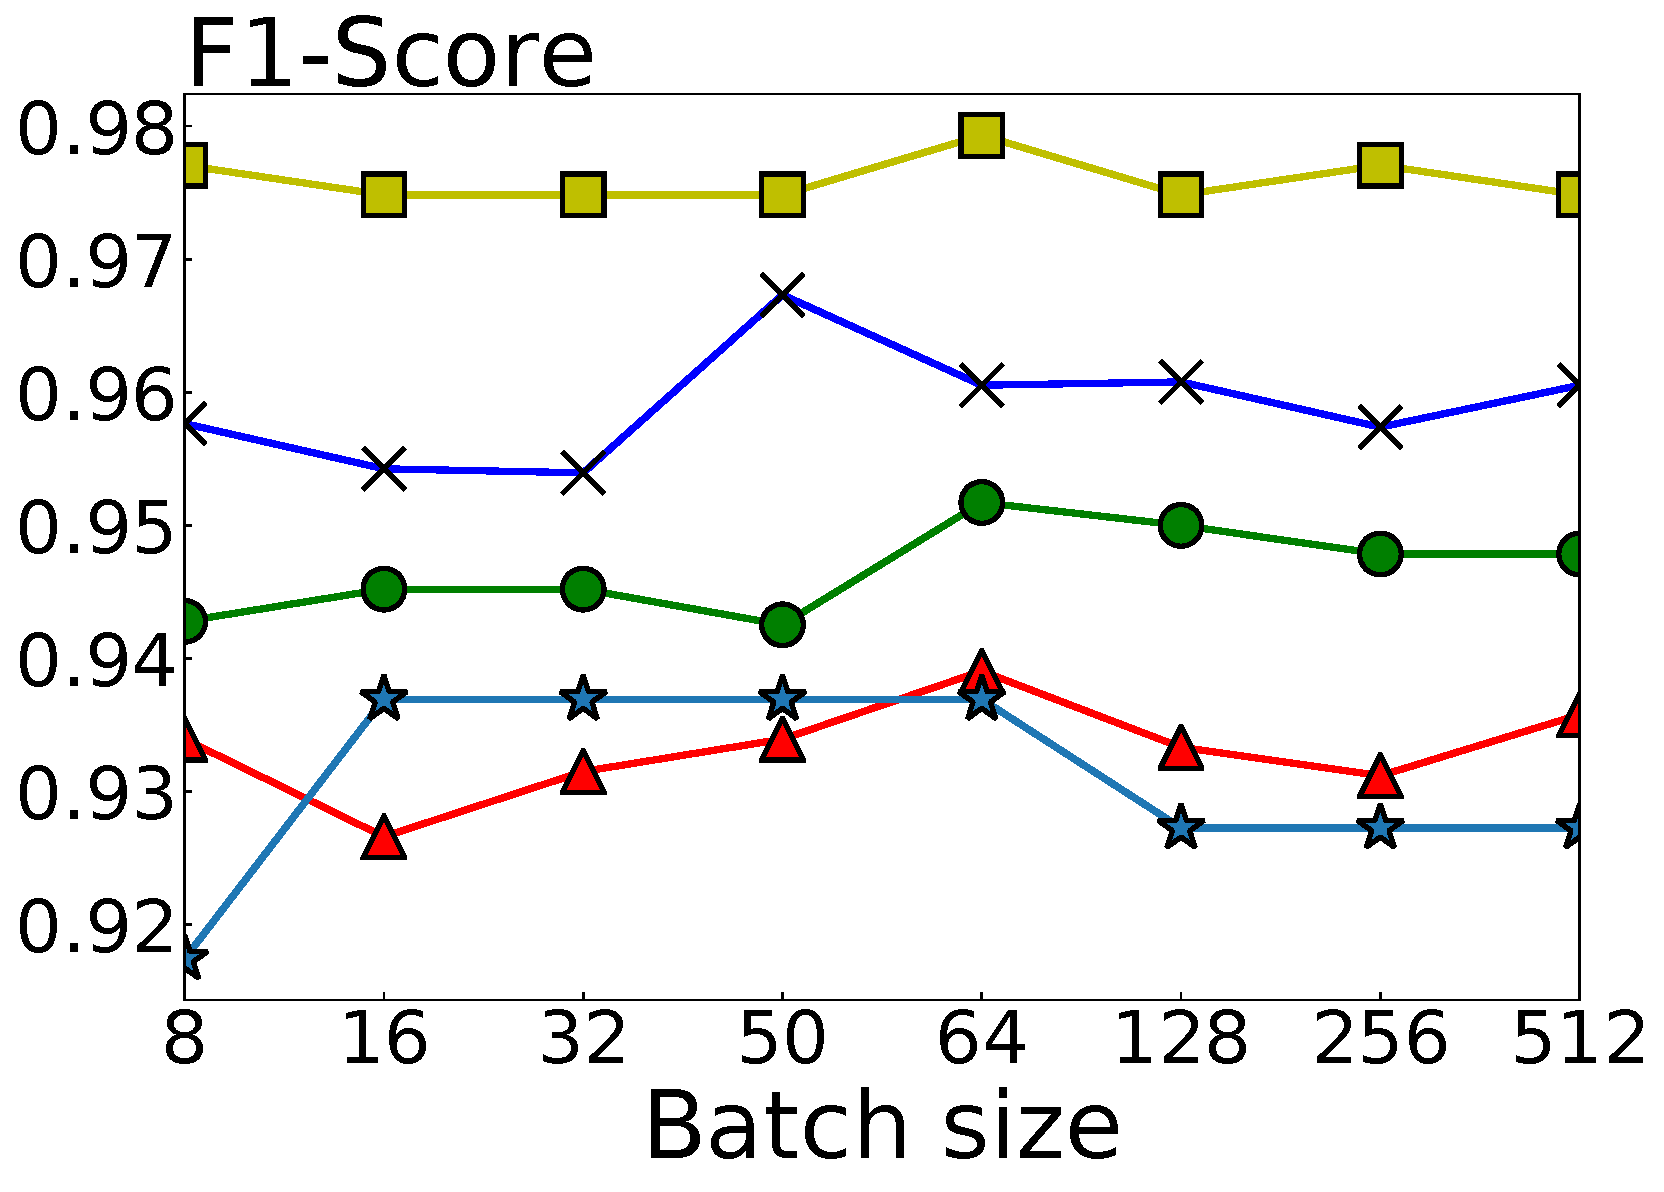
\includegraphics[width=1\linewidth]{fig/batch_size_events}
		\end{minipage}
		\begin{minipage}[b]{0.35\linewidth}
			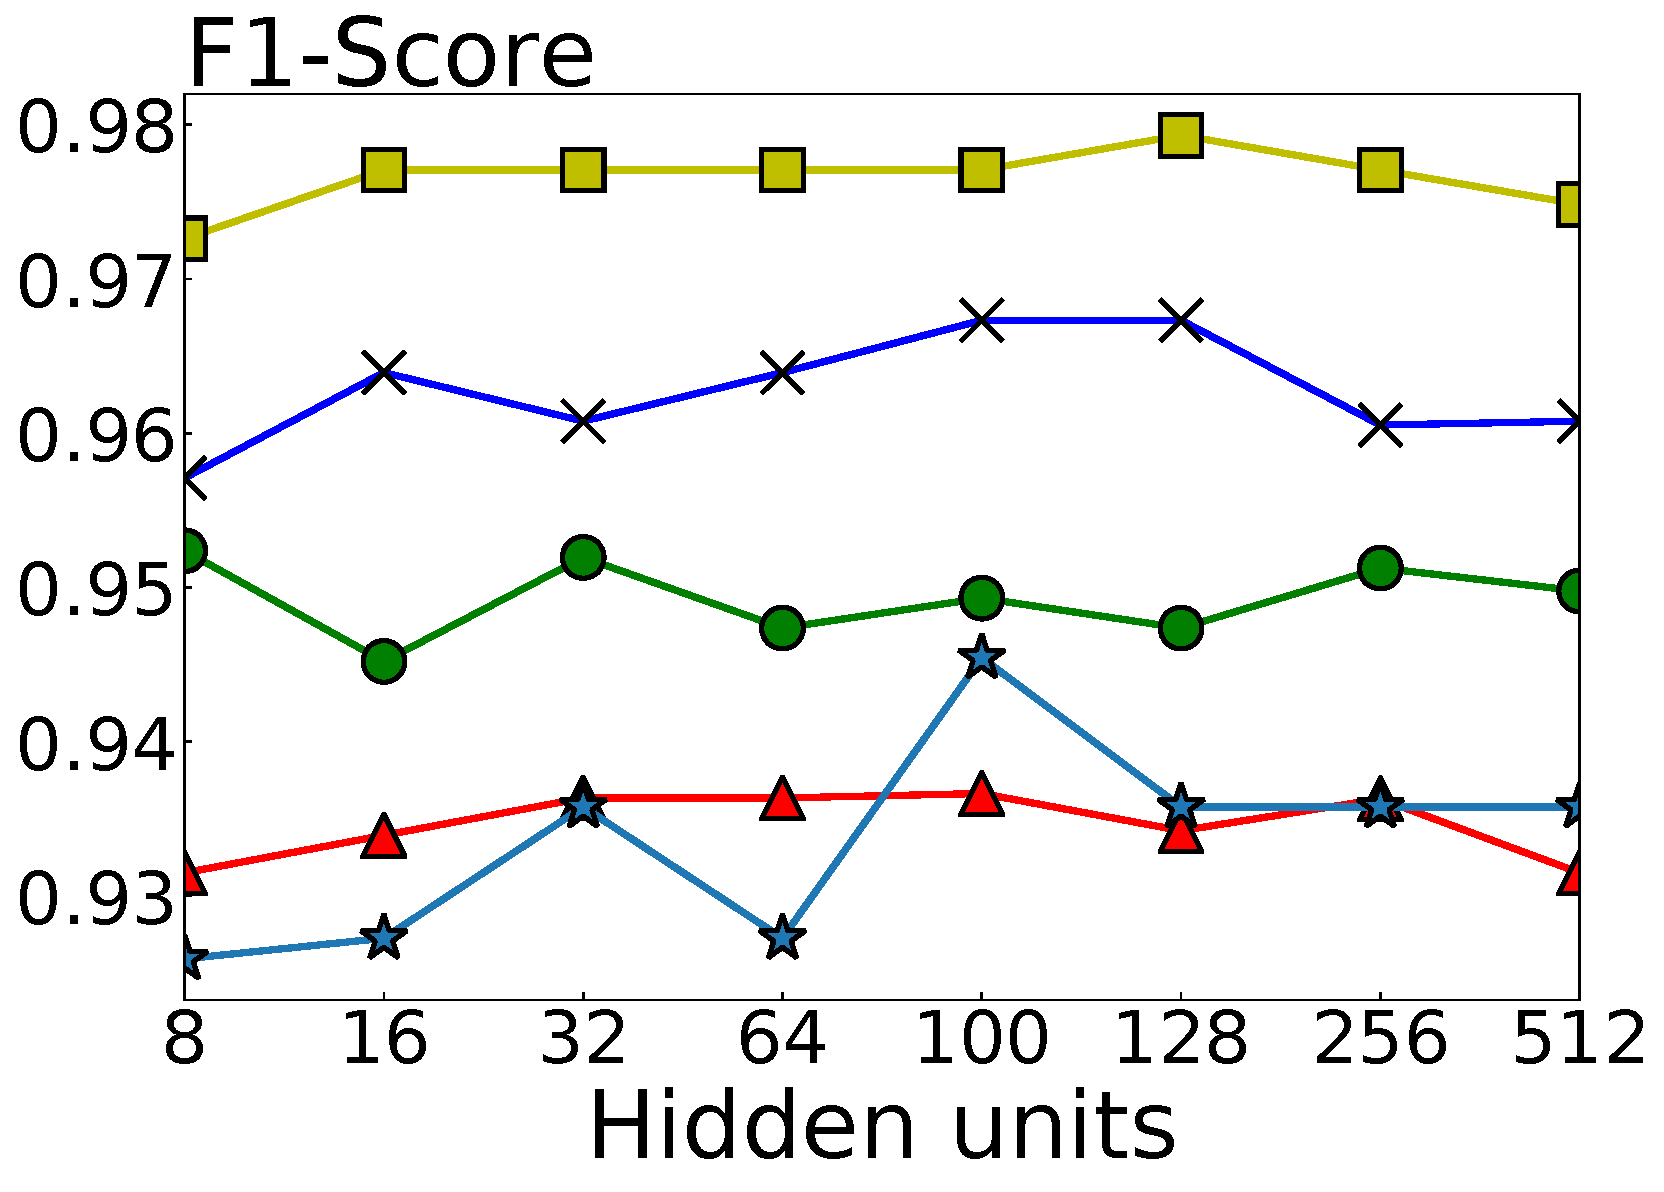
\includegraphics[width=1\linewidth]{fig/hidden_units_events}
		\end{minipage}
	}
	
	
	\subfigure{
		
\includegraphics[width=0.4\linewidth]{fig/legend_acc_macroF}
	}
	\setcounter{subfigure}{1}
	\subfigure[Affects of Parameters on F1-Scores and Accruancy]{
		\label{fig:parameter_art}
		\begin{minipage}[b]{0.35\linewidth}
			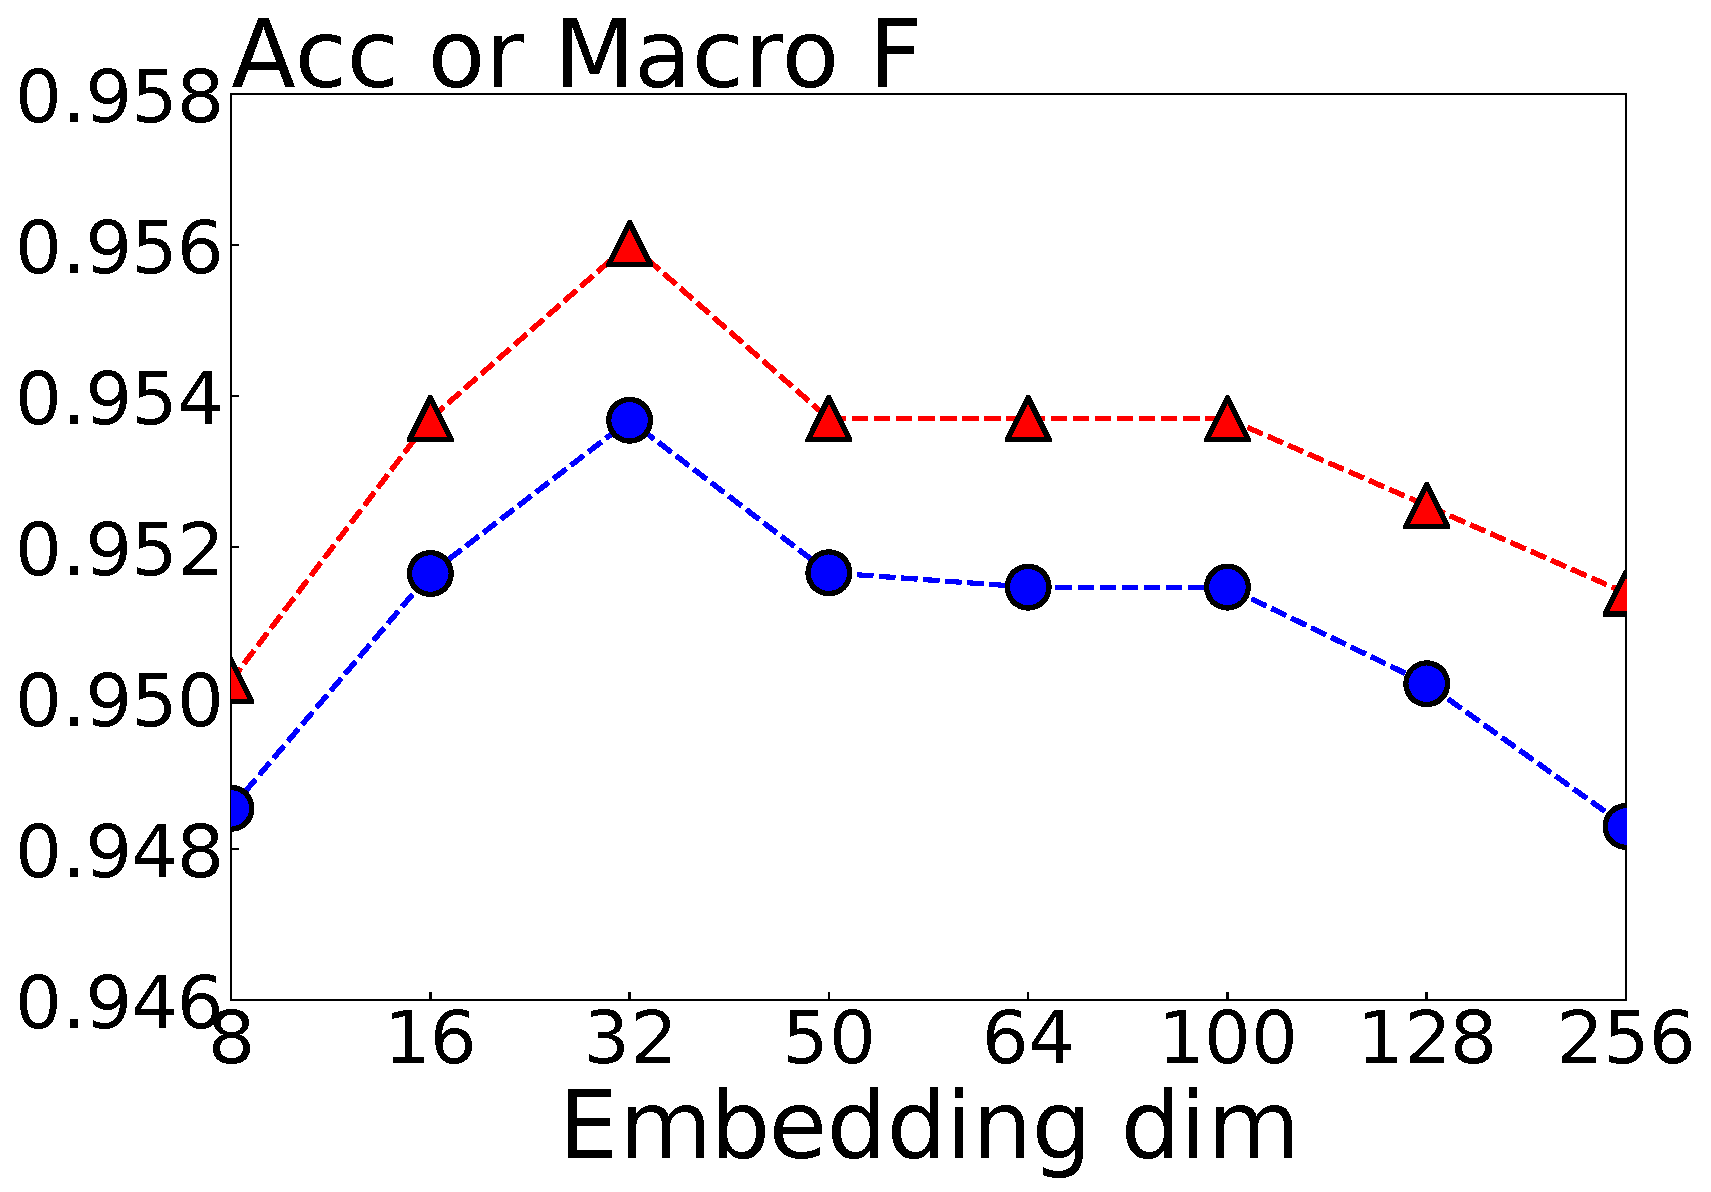
\includegraphics[width=1\linewidth]{fig/embedding_dim}
		\end{minipage}
		\begin{minipage}[b]{0.35\linewidth}
			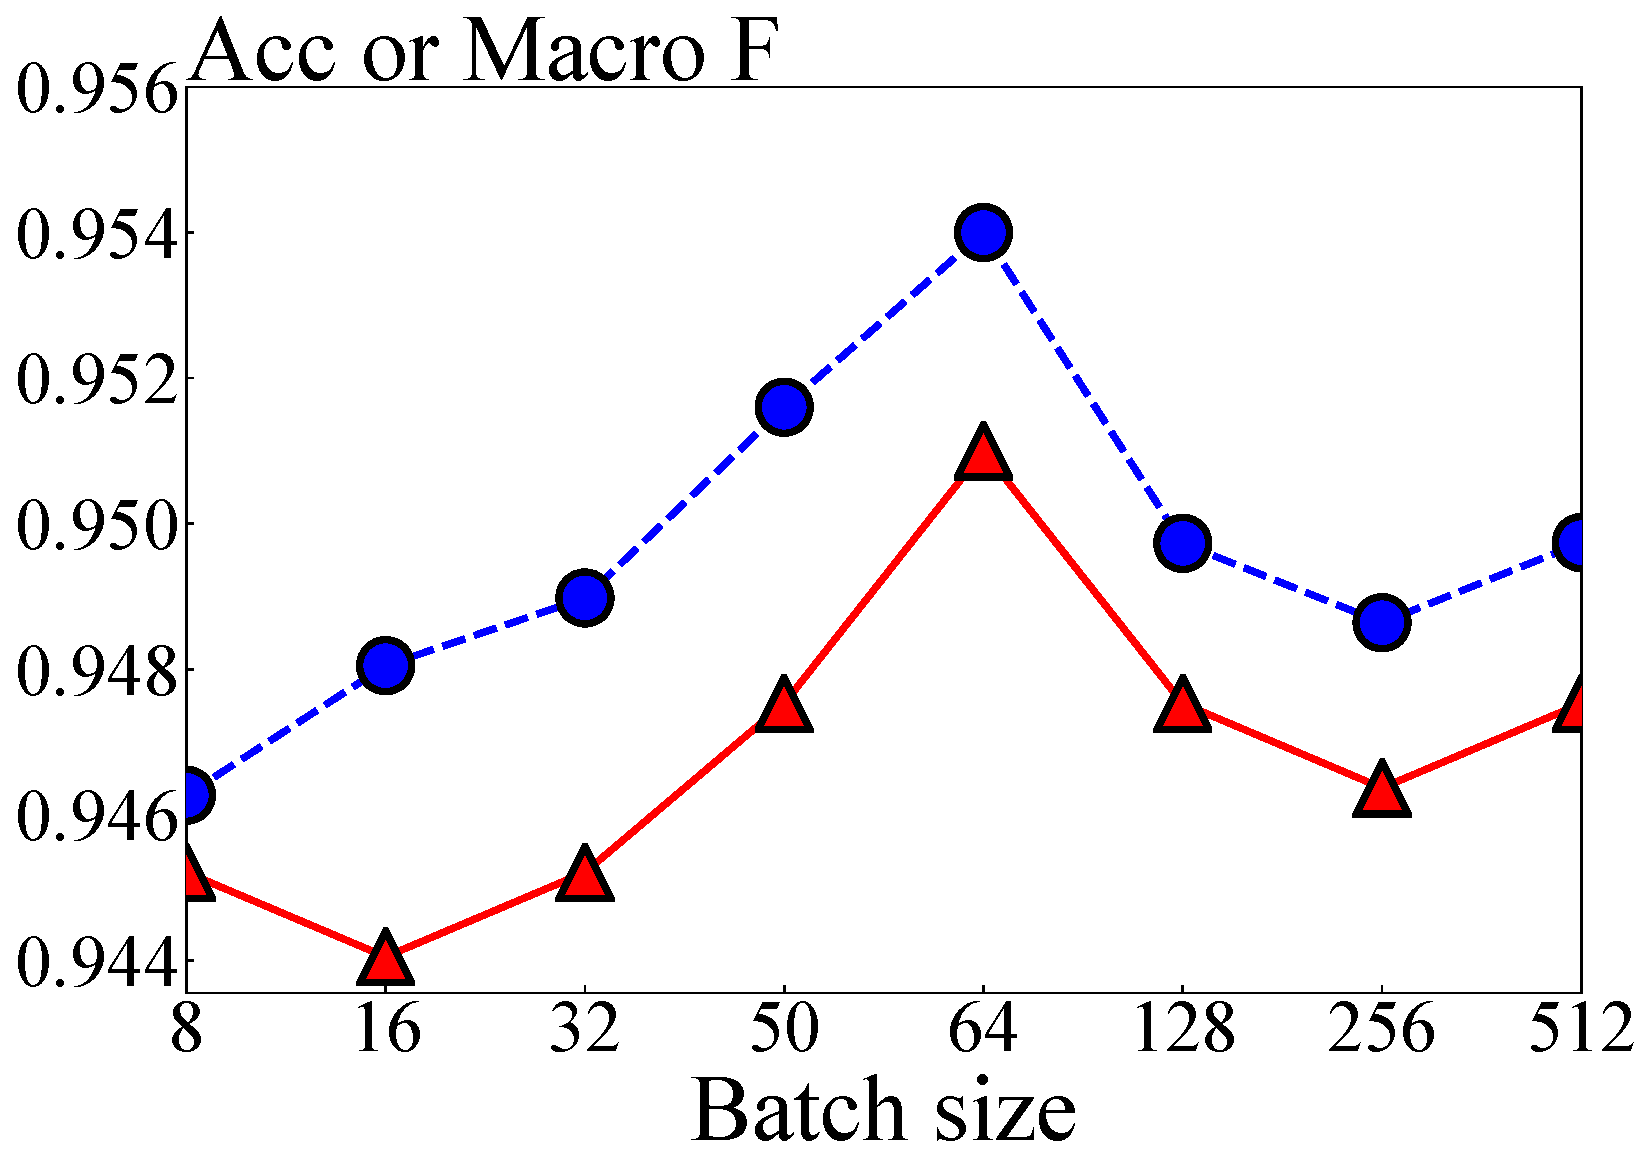
\includegraphics[width=1\linewidth]{fig/batch_size}
		\end{minipage}
		\begin{minipage}[b]{0.35\linewidth}
			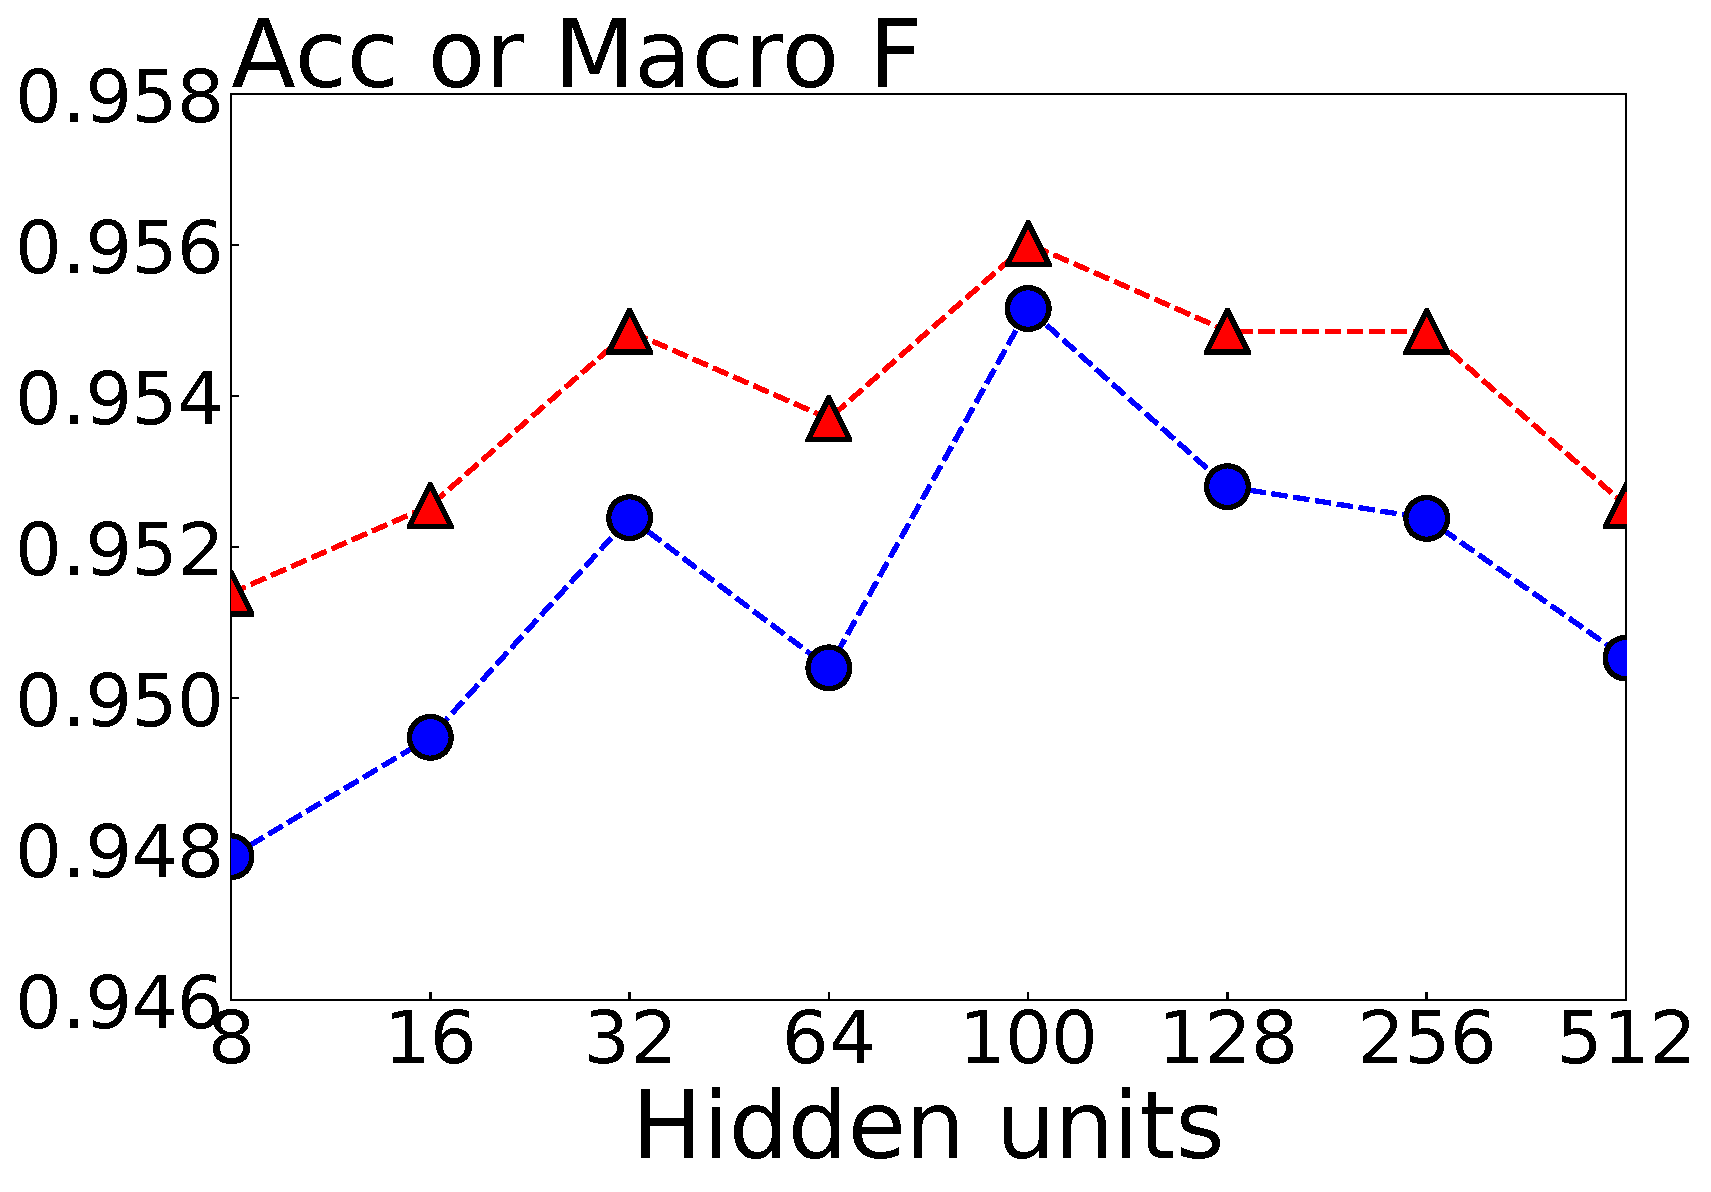
\includegraphics[width=1\linewidth]{fig/hidden_units}
		\end{minipage}
	}
	\caption{Adjustment of Parameters}
	\label{fig:parameter}
\end{figure}

\subsection{Details of Settings and Parameters}
In this part, we proceed to introduce the detailed settings of the experiments. The chosen optimizer in the deep learning based model is Adam. The loss function is cross-entropy. We split the whole dataset into a proportion of 6:2:2. For a deep learning based model, we  run it more than 50 epochs until convergence. Also, as shown in Fig.~\ref{fig:parameter}, we conduct various experiments to find the best parameters.

For simplicity, we only show the parameter adjustment on RumorEval as an example. We choose the embedding dimension, batch size, and hidden units as the representative parameters. During each running, we vary one parameter and fix the other parameters to record the variation trend of ART. The Fig.~\ref{fig:parameter_events} shows the results during parameter adjustment on each event. The Fig.~\ref{fig:parameter_art} records the performance of ART during parameter adjustment. It suggests that when the embedding dim is 32, batch size is 64, and hidden units is 100, the ART gets the best performance on RumorEval dataset. The smaller parameter value corresponds to the small scale of RumorEval.

\subsection{Discussion}
The experiments on baseline methods demonstrate the effectiveness of ART. ART outperforms the other models in most rumor events, showing robustness and superiority. The outstanding performance of the random embedding suggests that the pre-trained and the self-trained embeddings are not suitable in small-scaled dataset with causal spelling. Since some causal words is missing in pre-trained embeddings. Besides, the tweets is too short to train a satisfied self-trained embedding. The adjustment of the embedding dim shows that embeddings with small length is more suitable for rumor tracking. Because the long length embedding is spare, which brings additional computation. The comparison between basic model, pairwise-added models, and ART further demonstrates the effectiveness of ART. 


\section{Related Work}
\label{sec:related}

\subsection{Rumor Tracking}
\label{sec:rumortracking}
The earliest Rumor tracking work is traced back to 2011. Several studies aim to find the relevant rumors for a known prior \cite{DBLP:journals/csur/ZubiagaABLP18}. Qazvinian et al. \cite{DBLP:conf/emnlp/QazvinianRRM11} explores three types of features including content-based, network-based, and tweet specific memes for identifying rumors. Hamidian et al. \cite{DBLP:journals/corr/abs-1912-08926} devise novel features and classify rumors with WEKA platform. These studies all focus on building features with simple classifiers. Cheng et al. \cite{DBLP:conf/www/ChengNB20} propose a multi-task learning model named VRoC and treat rumor tracking as one of the sub-tasks. VRoC is based on variational auto-encoder and uses tweet content as the input features. Overall, the rumor tracking task is an important sub-task in rumor detection. However, compared to the other three sub-tasks, it attracts less attention.

\subsection{Text Classification}
\label{sec:textclassification}
Text classification is a significant task in the NLP area. In recent years, deep learning based text classification gets well developed. Kim et al. \cite{DBLP:conf/emnlp/Kim14} propose CNN based text classification. TextCNN uses different sized kernels to capture different scaled gram features. Bojanowski et al. propose FastText  \cite{DBLP:journals/tacl/BojanowskiGJM17}, which gets embeddings of text in a short time. Inception \cite{DBLP:journals/corr/SzegedyLJSRAEVR14} uses larger width of network structure to capture more features. DPCNN \cite{DBLP:conf/acl/JohnsonZ17} adopts a deeper network structure to get a better performance. From the recent studies, we find that the deep learning model achieves great success on text classification tasks.

\section{Conclusion}
\label{sec:conclusion}
Rumor Tracking is a valuable sub-task of automatically rumor defeating. In this paper, we propose a reinforcement learning based ensemble model named RL-ERT. We promote the performance of the rumor tracking task on accuracy and macro-F1 score with specific features and WTPN based ensemble strategy. Besides, well-designed experiments are carried out to demonstrate the effectiveness of RL-ERT. Experimental results on benchmark datasets suggest that our model outperforms the baseline methods by over 5\% on average. In the future, we will explore more efficient features for rumor detection, such as the links between users. Moreover, we consider utilizing the topology of social networks to promote the performance of rumor classifier.

\bibliography{mybibfile}

\end{document}